
% Default to the notebook output style

    


% Inherit from the specified cell style.




    
\documentclass[11pt]{article}

    
    
    \usepackage[T1]{fontenc}
    % Nicer default font (+ math font) than Computer Modern for most use cases
    \usepackage{mathpazo}

    % Basic figure setup, for now with no caption control since it's done
    % automatically by Pandoc (which extracts ![](path) syntax from Markdown).
    \usepackage{graphicx}
    % We will generate all images so they have a width \maxwidth. This means
    % that they will get their normal width if they fit onto the page, but
    % are scaled down if they would overflow the margins.
    \makeatletter
    \def\maxwidth{\ifdim\Gin@nat@width>\linewidth\linewidth
    \else\Gin@nat@width\fi}
    \makeatother
    \let\Oldincludegraphics\includegraphics
    % Set max figure width to be 80% of text width, for now hardcoded.
    \renewcommand{\includegraphics}[1]{\Oldincludegraphics[width=.8\maxwidth]{#1}}
    % Ensure that by default, figures have no caption (until we provide a
    % proper Figure object with a Caption API and a way to capture that
    % in the conversion process - todo).
    \usepackage{caption}
    \DeclareCaptionLabelFormat{nolabel}{}
    \captionsetup{labelformat=nolabel}

    \usepackage{adjustbox} % Used to constrain images to a maximum size 
    \usepackage{xcolor} % Allow colors to be defined
    \usepackage{enumerate} % Needed for markdown enumerations to work
    \usepackage{geometry} % Used to adjust the document margins
    \usepackage{amsmath} % Equations
    \usepackage{amssymb} % Equations
    \usepackage{textcomp} % defines textquotesingle
    % Hack from http://tex.stackexchange.com/a/47451/13684:
    \AtBeginDocument{%
        \def\PYZsq{\textquotesingle}% Upright quotes in Pygmentized code
    }
    \usepackage{upquote} % Upright quotes for verbatim code
    \usepackage{eurosym} % defines \euro
    \usepackage[mathletters]{ucs} % Extended unicode (utf-8) support
    \usepackage[utf8x]{inputenc} % Allow utf-8 characters in the tex document
    \usepackage{fancyvrb} % verbatim replacement that allows latex
    \usepackage{grffile} % extends the file name processing of package graphics 
                         % to support a larger range 
    % The hyperref package gives us a pdf with properly built
    % internal navigation ('pdf bookmarks' for the table of contents,
    % internal cross-reference links, web links for URLs, etc.)
    \usepackage{hyperref}
    \usepackage{longtable} % longtable support required by pandoc >1.10
    \usepackage{booktabs}  % table support for pandoc > 1.12.2
    \usepackage[inline]{enumitem} % IRkernel/repr support (it uses the enumerate* environment)
    \usepackage[normalem]{ulem} % ulem is needed to support strikethroughs (\sout)
                                % normalem makes italics be italics, not underlines
    

    
    
    % Colors for the hyperref package
    \definecolor{urlcolor}{rgb}{0,.145,.698}
    \definecolor{linkcolor}{rgb}{.71,0.21,0.01}
    \definecolor{citecolor}{rgb}{.12,.54,.11}

    % ANSI colors
    \definecolor{ansi-black}{HTML}{3E424D}
    \definecolor{ansi-black-intense}{HTML}{282C36}
    \definecolor{ansi-red}{HTML}{E75C58}
    \definecolor{ansi-red-intense}{HTML}{B22B31}
    \definecolor{ansi-green}{HTML}{00A250}
    \definecolor{ansi-green-intense}{HTML}{007427}
    \definecolor{ansi-yellow}{HTML}{DDB62B}
    \definecolor{ansi-yellow-intense}{HTML}{B27D12}
    \definecolor{ansi-blue}{HTML}{208FFB}
    \definecolor{ansi-blue-intense}{HTML}{0065CA}
    \definecolor{ansi-magenta}{HTML}{D160C4}
    \definecolor{ansi-magenta-intense}{HTML}{A03196}
    \definecolor{ansi-cyan}{HTML}{60C6C8}
    \definecolor{ansi-cyan-intense}{HTML}{258F8F}
    \definecolor{ansi-white}{HTML}{C5C1B4}
    \definecolor{ansi-white-intense}{HTML}{A1A6B2}

    % commands and environments needed by pandoc snippets
    % extracted from the output of `pandoc -s`
    \providecommand{\tightlist}{%
      \setlength{\itemsep}{0pt}\setlength{\parskip}{0pt}}
    \DefineVerbatimEnvironment{Highlighting}{Verbatim}{commandchars=\\\{\}}
    % Add ',fontsize=\small' for more characters per line
    \newenvironment{Shaded}{}{}
    \newcommand{\KeywordTok}[1]{\textcolor[rgb]{0.00,0.44,0.13}{\textbf{{#1}}}}
    \newcommand{\DataTypeTok}[1]{\textcolor[rgb]{0.56,0.13,0.00}{{#1}}}
    \newcommand{\DecValTok}[1]{\textcolor[rgb]{0.25,0.63,0.44}{{#1}}}
    \newcommand{\BaseNTok}[1]{\textcolor[rgb]{0.25,0.63,0.44}{{#1}}}
    \newcommand{\FloatTok}[1]{\textcolor[rgb]{0.25,0.63,0.44}{{#1}}}
    \newcommand{\CharTok}[1]{\textcolor[rgb]{0.25,0.44,0.63}{{#1}}}
    \newcommand{\StringTok}[1]{\textcolor[rgb]{0.25,0.44,0.63}{{#1}}}
    \newcommand{\CommentTok}[1]{\textcolor[rgb]{0.38,0.63,0.69}{\textit{{#1}}}}
    \newcommand{\OtherTok}[1]{\textcolor[rgb]{0.00,0.44,0.13}{{#1}}}
    \newcommand{\AlertTok}[1]{\textcolor[rgb]{1.00,0.00,0.00}{\textbf{{#1}}}}
    \newcommand{\FunctionTok}[1]{\textcolor[rgb]{0.02,0.16,0.49}{{#1}}}
    \newcommand{\RegionMarkerTok}[1]{{#1}}
    \newcommand{\ErrorTok}[1]{\textcolor[rgb]{1.00,0.00,0.00}{\textbf{{#1}}}}
    \newcommand{\NormalTok}[1]{{#1}}
    
    % Additional commands for more recent versions of Pandoc
    \newcommand{\ConstantTok}[1]{\textcolor[rgb]{0.53,0.00,0.00}{{#1}}}
    \newcommand{\SpecialCharTok}[1]{\textcolor[rgb]{0.25,0.44,0.63}{{#1}}}
    \newcommand{\VerbatimStringTok}[1]{\textcolor[rgb]{0.25,0.44,0.63}{{#1}}}
    \newcommand{\SpecialStringTok}[1]{\textcolor[rgb]{0.73,0.40,0.53}{{#1}}}
    \newcommand{\ImportTok}[1]{{#1}}
    \newcommand{\DocumentationTok}[1]{\textcolor[rgb]{0.73,0.13,0.13}{\textit{{#1}}}}
    \newcommand{\AnnotationTok}[1]{\textcolor[rgb]{0.38,0.63,0.69}{\textbf{\textit{{#1}}}}}
    \newcommand{\CommentVarTok}[1]{\textcolor[rgb]{0.38,0.63,0.69}{\textbf{\textit{{#1}}}}}
    \newcommand{\VariableTok}[1]{\textcolor[rgb]{0.10,0.09,0.49}{{#1}}}
    \newcommand{\ControlFlowTok}[1]{\textcolor[rgb]{0.00,0.44,0.13}{\textbf{{#1}}}}
    \newcommand{\OperatorTok}[1]{\textcolor[rgb]{0.40,0.40,0.40}{{#1}}}
    \newcommand{\BuiltInTok}[1]{{#1}}
    \newcommand{\ExtensionTok}[1]{{#1}}
    \newcommand{\PreprocessorTok}[1]{\textcolor[rgb]{0.74,0.48,0.00}{{#1}}}
    \newcommand{\AttributeTok}[1]{\textcolor[rgb]{0.49,0.56,0.16}{{#1}}}
    \newcommand{\InformationTok}[1]{\textcolor[rgb]{0.38,0.63,0.69}{\textbf{\textit{{#1}}}}}
    \newcommand{\WarningTok}[1]{\textcolor[rgb]{0.38,0.63,0.69}{\textbf{\textit{{#1}}}}}
    
    
    % Define a nice break command that doesn't care if a line doesn't already
    % exist.
    \def\br{\hspace*{\fill} \\* }
    % Math Jax compatability definitions
    \def\gt{>}
    \def\lt{<}
    % Document parameters
    \title{ECCO\_v4\_A\_Better\_Method\_for\_Loading\_ECCOv4\_NetCDF\_Tile\_Files}
    
    
    

    % Pygments definitions
    
\makeatletter
\def\PY@reset{\let\PY@it=\relax \let\PY@bf=\relax%
    \let\PY@ul=\relax \let\PY@tc=\relax%
    \let\PY@bc=\relax \let\PY@ff=\relax}
\def\PY@tok#1{\csname PY@tok@#1\endcsname}
\def\PY@toks#1+{\ifx\relax#1\empty\else%
    \PY@tok{#1}\expandafter\PY@toks\fi}
\def\PY@do#1{\PY@bc{\PY@tc{\PY@ul{%
    \PY@it{\PY@bf{\PY@ff{#1}}}}}}}
\def\PY#1#2{\PY@reset\PY@toks#1+\relax+\PY@do{#2}}

\expandafter\def\csname PY@tok@gd\endcsname{\def\PY@tc##1{\textcolor[rgb]{0.63,0.00,0.00}{##1}}}
\expandafter\def\csname PY@tok@gu\endcsname{\let\PY@bf=\textbf\def\PY@tc##1{\textcolor[rgb]{0.50,0.00,0.50}{##1}}}
\expandafter\def\csname PY@tok@gt\endcsname{\def\PY@tc##1{\textcolor[rgb]{0.00,0.27,0.87}{##1}}}
\expandafter\def\csname PY@tok@gs\endcsname{\let\PY@bf=\textbf}
\expandafter\def\csname PY@tok@gr\endcsname{\def\PY@tc##1{\textcolor[rgb]{1.00,0.00,0.00}{##1}}}
\expandafter\def\csname PY@tok@cm\endcsname{\let\PY@it=\textit\def\PY@tc##1{\textcolor[rgb]{0.25,0.50,0.50}{##1}}}
\expandafter\def\csname PY@tok@vg\endcsname{\def\PY@tc##1{\textcolor[rgb]{0.10,0.09,0.49}{##1}}}
\expandafter\def\csname PY@tok@vi\endcsname{\def\PY@tc##1{\textcolor[rgb]{0.10,0.09,0.49}{##1}}}
\expandafter\def\csname PY@tok@vm\endcsname{\def\PY@tc##1{\textcolor[rgb]{0.10,0.09,0.49}{##1}}}
\expandafter\def\csname PY@tok@mh\endcsname{\def\PY@tc##1{\textcolor[rgb]{0.40,0.40,0.40}{##1}}}
\expandafter\def\csname PY@tok@cs\endcsname{\let\PY@it=\textit\def\PY@tc##1{\textcolor[rgb]{0.25,0.50,0.50}{##1}}}
\expandafter\def\csname PY@tok@ge\endcsname{\let\PY@it=\textit}
\expandafter\def\csname PY@tok@vc\endcsname{\def\PY@tc##1{\textcolor[rgb]{0.10,0.09,0.49}{##1}}}
\expandafter\def\csname PY@tok@il\endcsname{\def\PY@tc##1{\textcolor[rgb]{0.40,0.40,0.40}{##1}}}
\expandafter\def\csname PY@tok@go\endcsname{\def\PY@tc##1{\textcolor[rgb]{0.53,0.53,0.53}{##1}}}
\expandafter\def\csname PY@tok@cp\endcsname{\def\PY@tc##1{\textcolor[rgb]{0.74,0.48,0.00}{##1}}}
\expandafter\def\csname PY@tok@gi\endcsname{\def\PY@tc##1{\textcolor[rgb]{0.00,0.63,0.00}{##1}}}
\expandafter\def\csname PY@tok@gh\endcsname{\let\PY@bf=\textbf\def\PY@tc##1{\textcolor[rgb]{0.00,0.00,0.50}{##1}}}
\expandafter\def\csname PY@tok@ni\endcsname{\let\PY@bf=\textbf\def\PY@tc##1{\textcolor[rgb]{0.60,0.60,0.60}{##1}}}
\expandafter\def\csname PY@tok@nl\endcsname{\def\PY@tc##1{\textcolor[rgb]{0.63,0.63,0.00}{##1}}}
\expandafter\def\csname PY@tok@nn\endcsname{\let\PY@bf=\textbf\def\PY@tc##1{\textcolor[rgb]{0.00,0.00,1.00}{##1}}}
\expandafter\def\csname PY@tok@no\endcsname{\def\PY@tc##1{\textcolor[rgb]{0.53,0.00,0.00}{##1}}}
\expandafter\def\csname PY@tok@na\endcsname{\def\PY@tc##1{\textcolor[rgb]{0.49,0.56,0.16}{##1}}}
\expandafter\def\csname PY@tok@nb\endcsname{\def\PY@tc##1{\textcolor[rgb]{0.00,0.50,0.00}{##1}}}
\expandafter\def\csname PY@tok@nc\endcsname{\let\PY@bf=\textbf\def\PY@tc##1{\textcolor[rgb]{0.00,0.00,1.00}{##1}}}
\expandafter\def\csname PY@tok@nd\endcsname{\def\PY@tc##1{\textcolor[rgb]{0.67,0.13,1.00}{##1}}}
\expandafter\def\csname PY@tok@ne\endcsname{\let\PY@bf=\textbf\def\PY@tc##1{\textcolor[rgb]{0.82,0.25,0.23}{##1}}}
\expandafter\def\csname PY@tok@nf\endcsname{\def\PY@tc##1{\textcolor[rgb]{0.00,0.00,1.00}{##1}}}
\expandafter\def\csname PY@tok@si\endcsname{\let\PY@bf=\textbf\def\PY@tc##1{\textcolor[rgb]{0.73,0.40,0.53}{##1}}}
\expandafter\def\csname PY@tok@s2\endcsname{\def\PY@tc##1{\textcolor[rgb]{0.73,0.13,0.13}{##1}}}
\expandafter\def\csname PY@tok@nt\endcsname{\let\PY@bf=\textbf\def\PY@tc##1{\textcolor[rgb]{0.00,0.50,0.00}{##1}}}
\expandafter\def\csname PY@tok@nv\endcsname{\def\PY@tc##1{\textcolor[rgb]{0.10,0.09,0.49}{##1}}}
\expandafter\def\csname PY@tok@s1\endcsname{\def\PY@tc##1{\textcolor[rgb]{0.73,0.13,0.13}{##1}}}
\expandafter\def\csname PY@tok@dl\endcsname{\def\PY@tc##1{\textcolor[rgb]{0.73,0.13,0.13}{##1}}}
\expandafter\def\csname PY@tok@ch\endcsname{\let\PY@it=\textit\def\PY@tc##1{\textcolor[rgb]{0.25,0.50,0.50}{##1}}}
\expandafter\def\csname PY@tok@m\endcsname{\def\PY@tc##1{\textcolor[rgb]{0.40,0.40,0.40}{##1}}}
\expandafter\def\csname PY@tok@gp\endcsname{\let\PY@bf=\textbf\def\PY@tc##1{\textcolor[rgb]{0.00,0.00,0.50}{##1}}}
\expandafter\def\csname PY@tok@sh\endcsname{\def\PY@tc##1{\textcolor[rgb]{0.73,0.13,0.13}{##1}}}
\expandafter\def\csname PY@tok@ow\endcsname{\let\PY@bf=\textbf\def\PY@tc##1{\textcolor[rgb]{0.67,0.13,1.00}{##1}}}
\expandafter\def\csname PY@tok@sx\endcsname{\def\PY@tc##1{\textcolor[rgb]{0.00,0.50,0.00}{##1}}}
\expandafter\def\csname PY@tok@bp\endcsname{\def\PY@tc##1{\textcolor[rgb]{0.00,0.50,0.00}{##1}}}
\expandafter\def\csname PY@tok@c1\endcsname{\let\PY@it=\textit\def\PY@tc##1{\textcolor[rgb]{0.25,0.50,0.50}{##1}}}
\expandafter\def\csname PY@tok@fm\endcsname{\def\PY@tc##1{\textcolor[rgb]{0.00,0.00,1.00}{##1}}}
\expandafter\def\csname PY@tok@o\endcsname{\def\PY@tc##1{\textcolor[rgb]{0.40,0.40,0.40}{##1}}}
\expandafter\def\csname PY@tok@kc\endcsname{\let\PY@bf=\textbf\def\PY@tc##1{\textcolor[rgb]{0.00,0.50,0.00}{##1}}}
\expandafter\def\csname PY@tok@c\endcsname{\let\PY@it=\textit\def\PY@tc##1{\textcolor[rgb]{0.25,0.50,0.50}{##1}}}
\expandafter\def\csname PY@tok@mf\endcsname{\def\PY@tc##1{\textcolor[rgb]{0.40,0.40,0.40}{##1}}}
\expandafter\def\csname PY@tok@err\endcsname{\def\PY@bc##1{\setlength{\fboxsep}{0pt}\fcolorbox[rgb]{1.00,0.00,0.00}{1,1,1}{\strut ##1}}}
\expandafter\def\csname PY@tok@mb\endcsname{\def\PY@tc##1{\textcolor[rgb]{0.40,0.40,0.40}{##1}}}
\expandafter\def\csname PY@tok@ss\endcsname{\def\PY@tc##1{\textcolor[rgb]{0.10,0.09,0.49}{##1}}}
\expandafter\def\csname PY@tok@sr\endcsname{\def\PY@tc##1{\textcolor[rgb]{0.73,0.40,0.53}{##1}}}
\expandafter\def\csname PY@tok@mo\endcsname{\def\PY@tc##1{\textcolor[rgb]{0.40,0.40,0.40}{##1}}}
\expandafter\def\csname PY@tok@kd\endcsname{\let\PY@bf=\textbf\def\PY@tc##1{\textcolor[rgb]{0.00,0.50,0.00}{##1}}}
\expandafter\def\csname PY@tok@mi\endcsname{\def\PY@tc##1{\textcolor[rgb]{0.40,0.40,0.40}{##1}}}
\expandafter\def\csname PY@tok@kn\endcsname{\let\PY@bf=\textbf\def\PY@tc##1{\textcolor[rgb]{0.00,0.50,0.00}{##1}}}
\expandafter\def\csname PY@tok@cpf\endcsname{\let\PY@it=\textit\def\PY@tc##1{\textcolor[rgb]{0.25,0.50,0.50}{##1}}}
\expandafter\def\csname PY@tok@kr\endcsname{\let\PY@bf=\textbf\def\PY@tc##1{\textcolor[rgb]{0.00,0.50,0.00}{##1}}}
\expandafter\def\csname PY@tok@s\endcsname{\def\PY@tc##1{\textcolor[rgb]{0.73,0.13,0.13}{##1}}}
\expandafter\def\csname PY@tok@kp\endcsname{\def\PY@tc##1{\textcolor[rgb]{0.00,0.50,0.00}{##1}}}
\expandafter\def\csname PY@tok@w\endcsname{\def\PY@tc##1{\textcolor[rgb]{0.73,0.73,0.73}{##1}}}
\expandafter\def\csname PY@tok@kt\endcsname{\def\PY@tc##1{\textcolor[rgb]{0.69,0.00,0.25}{##1}}}
\expandafter\def\csname PY@tok@sc\endcsname{\def\PY@tc##1{\textcolor[rgb]{0.73,0.13,0.13}{##1}}}
\expandafter\def\csname PY@tok@sb\endcsname{\def\PY@tc##1{\textcolor[rgb]{0.73,0.13,0.13}{##1}}}
\expandafter\def\csname PY@tok@sa\endcsname{\def\PY@tc##1{\textcolor[rgb]{0.73,0.13,0.13}{##1}}}
\expandafter\def\csname PY@tok@k\endcsname{\let\PY@bf=\textbf\def\PY@tc##1{\textcolor[rgb]{0.00,0.50,0.00}{##1}}}
\expandafter\def\csname PY@tok@se\endcsname{\let\PY@bf=\textbf\def\PY@tc##1{\textcolor[rgb]{0.73,0.40,0.13}{##1}}}
\expandafter\def\csname PY@tok@sd\endcsname{\let\PY@it=\textit\def\PY@tc##1{\textcolor[rgb]{0.73,0.13,0.13}{##1}}}

\def\PYZbs{\char`\\}
\def\PYZus{\char`\_}
\def\PYZob{\char`\{}
\def\PYZcb{\char`\}}
\def\PYZca{\char`\^}
\def\PYZam{\char`\&}
\def\PYZlt{\char`\<}
\def\PYZgt{\char`\>}
\def\PYZsh{\char`\#}
\def\PYZpc{\char`\%}
\def\PYZdl{\char`\$}
\def\PYZhy{\char`\-}
\def\PYZsq{\char`\'}
\def\PYZdq{\char`\"}
\def\PYZti{\char`\~}
% for compatibility with earlier versions
\def\PYZat{@}
\def\PYZlb{[}
\def\PYZrb{]}
\makeatother


    % Exact colors from NB
    \definecolor{incolor}{rgb}{0.0, 0.0, 0.5}
    \definecolor{outcolor}{rgb}{0.545, 0.0, 0.0}



    
    % Prevent overflowing lines due to hard-to-break entities
    \sloppy 
    % Setup hyperref package
    \hypersetup{
      breaklinks=true,  % so long urls are correctly broken across lines
      colorlinks=true,
      urlcolor=urlcolor,
      linkcolor=linkcolor,
      citecolor=citecolor,
      }
    % Slightly bigger margins than the latex defaults
    
    \geometry{verbose,tmargin=1in,bmargin=1in,lmargin=1in,rmargin=1in}
    
    

    \begin{document}
    
    
    \maketitle
    
    

    
    \section{A Better Method for Loading ECCOv4 NetCDF Tile
Files}\label{a-better-method-for-loading-eccov4-netcdf-tile-files}

\subsection{Objectives:}\label{objectives}

Introduce an alternative method for loading ECCO v4 NetCDF tile files
that returns \texttt{Dataset} and \texttt{DataArray} objects with better
labelling of variable coordinates with respect to \emph{where} they are
situated on the Arakawa-C grid.

\subsection{Introduction}\label{introduction}

As we showed in the first tutorial, we can use the
\texttt{open\_dataset} method from \texttt{xarray} to load a NetCDF tile
file into Python as a \texttt{Dataset} object. \texttt{open\_dataset} is
very convienent because it automatically parses the NetCDF file and
constructs a \texttt{Dataset} object using all of the dimensions,
coordinates, variables, and metadata information. However, by default
the names of the coordinates are pretty generic: \textbf{i1, i2, i3},
etc. We can do a lot better.

In the last tutorial we loaded a single ECCOv4 grid tile file and
examined its contents. Let's load it up again and take another look at
its coordinates. This time we'll name the new \texttt{Dataset} object
\texttt{grid\_3\_od} since we are loading the file using
\texttt{open\_dataset}.

    \begin{Verbatim}[commandchars=\\\{\}]
{\color{incolor}In [{\color{incolor}68}]:} \PY{k+kn}{import} \PY{n+nn}{matplotlib.pylab} \PY{k+kn}{as} \PY{n+nn}{plt}
         \PY{k+kn}{import} \PY{n+nn}{numpy} \PY{k+kn}{as} \PY{n+nn}{np}
         \PY{k+kn}{import} \PY{n+nn}{sys}
         \PY{k+kn}{import} \PY{n+nn}{xarray} \PY{k+kn}{as} \PY{n+nn}{xr}
         \PY{k+kn}{from} \PY{n+nn}{copy} \PY{k+kn}{import} \PY{n}{deepcopy} 
         \PY{k+kn}{import} \PY{n+nn}{ecco\PYZus{}v4\PYZus{}py} \PY{k+kn}{as} \PY{n+nn}{ecco}
\end{Verbatim}


    \begin{Verbatim}[commandchars=\\\{\}]
{\color{incolor}In [{\color{incolor}69}]:} \PY{c+c1}{\PYZsh{} point to your local directory holding the nctiles\PYZus{}grid files}
         \PY{n}{grid\PYZus{}dir}\PY{o}{=}\PY{l+s+s1}{\PYZsq{}}\PY{l+s+s1}{/Volumes/ECCO\PYZus{}BASE/ECCO\PYZus{}v4r3/nctiles\PYZus{}grid/}\PY{l+s+s1}{\PYZsq{}}
         \PY{n}{fname} \PY{o}{=} \PY{l+s+s1}{\PYZsq{}}\PY{l+s+s1}{GRID.0003.nc}\PY{l+s+s1}{\PYZsq{}}
         \PY{n}{grid\PYZus{}3\PYZus{}od} \PY{o}{=} \PY{n}{xr}\PY{o}{.}\PY{n}{open\PYZus{}dataset}\PY{p}{(}\PY{n}{grid\PYZus{}dir} \PY{o}{+} \PY{n}{fname}\PY{p}{)}
\end{Verbatim}


    \begin{Verbatim}[commandchars=\\\{\}]
{\color{incolor}In [{\color{incolor}70}]:} \PY{n}{grid\PYZus{}3\PYZus{}od}
\end{Verbatim}


\begin{Verbatim}[commandchars=\\\{\}]
{\color{outcolor}Out[{\color{outcolor}70}]:} <xarray.Dataset>
         Dimensions:  (i1: 50, i2: 90, i3: 90)
         Coordinates:
           * i1       (i1) float64 1.0 2.0 3.0 4.0 5.0 6.0 7.0 8.0 9.0 10.0 11.0 12.0 {\ldots}
           * i2       (i2) float64 1.0 2.0 3.0 4.0 5.0 6.0 7.0 8.0 9.0 10.0 11.0 12.0 {\ldots}
           * i3       (i3) float64 1.0 2.0 3.0 4.0 5.0 6.0 7.0 8.0 9.0 10.0 11.0 12.0 {\ldots}
         Data variables:
             hFacC    (i1, i2, i3) float64 {\ldots}
             hFacW    (i1, i2, i3) float64 {\ldots}
             hFacS    (i1, i2, i3) float64 {\ldots}
             XC       (i2, i3) float64 {\ldots}
             YC       (i2, i3) float64 {\ldots}
             XG       (i2, i3) float64 {\ldots}
             YG       (i2, i3) float64 {\ldots}
             RAC      (i2, i3) float64 {\ldots}
             RAZ      (i2, i3) float64 {\ldots}
             DXC      (i2, i3) float64 {\ldots}
             DYC      (i2, i3) float64 {\ldots}
             DXG      (i2, i3) float64 {\ldots}
             DYG      (i2, i3) float64 {\ldots}
             Depth    (i2, i3) float64 {\ldots}
             AngleCS  (i2, i3) float64 {\ldots}
             AngleSN  (i2, i3) float64 {\ldots}
             RC       (i1) float64 {\ldots}
             RF       (i1) float64 {\ldots}
             DRC      (i1) float64 {\ldots}
             DRF      (i1) float64 {\ldots}
         Attributes:
             description:    C-grid parameters (see MITgcm documentation for details){\ldots}
             A:              :Format      = native grid (nctiles w. 13 tiles)
             B:              :source      = ECCO consortium (http://ecco-group.org/)
             C:              :institution = JPL/UT/MIT/AER
             D:              :history     = files revision history :
             E:                                 04/20/2017: fill in geometry info for {\ldots}
             F:                                 11/06/2016: third release of ECCO v4 ({\ldots}
             G:                             estimates revision history (from second re{\ldots}
             H:                                 employs bi-harmonic viscosity (enhance{\ldots}
             I:                                 sea-ice parameters, updated or novel o{\ldots}
             J:                                 GRACE OBP, Aquarius SSS, global mean s{\ldots}
             K:                                 time-series, extended and/or expanded {\ldots}
             L:                                 revised weights including data and con{\ldots}
             M:                                 to account for grid-size variation and{\ldots}
             N:                                 separate time-mean and time-variable d{\ldots}
             O:                                 and controls, sea-ice costs, and initi{\ldots}
             P:                                 additional controls.\textbackslash{}n 
             Q:              :references  = Forget, G., J.-M. Campin, P. Heimbach, C. {\ldots}
             R:                              and C. Wunsch, 2015: ECCO version 4: an i{\ldots}
             S:                              non-linear inverse modeling and global oc{\ldots}
             T:                              Geoscientific Model Development, 8, 3071-{\ldots}
             U:                             Forget, G., J.-M. Campin, P. Heimbach, C. {\ldots}
             V:                              ECCO version 4: Second Release, 2016, htt{\ldots}
             W:              file created using gcmfaces\_IO/write2nctiles.m
             date:           21-Apr-2017
             Conventions:    CF-1.6
             \_FillValue:     nan
             missing\_value:  nan
\end{Verbatim}
            
    \subsubsection{Examining the Dataset object
contents}\label{examining-the-dataset-object-contents}

We see that all of the Data variables in \texttt{grid\_3\_od} use one of
three dimensions, \textbf{i1}, \textbf{i2}, and \textbf{i3}. As we saw
before, some variables are 3D, \(hFacC(i1,i2,i3)\); others are 2D,
\(XC(i2,i3)\); and others are 1D, \(RF(i1)\).

While this \texttt{Dataset} object is useful, its coordinate names are
somewhat ambiguous. The MITgcm uses the staggered Arakawa-C grid
(hereafter c-grid) to discretize the model equations. Model variables
are not co-located in c-grid models; they can fall on one of four
different categories of point. From the above, one cannot distinguish
\emph{where} on the \emph{c-grid} these different variables are
situated.

To understand this issue better, let's review the c-grid coordinate
system.

\subsection{The four horizontal points of the
c-grid}\label{the-four-horizontal-points-of-the-c-grid}

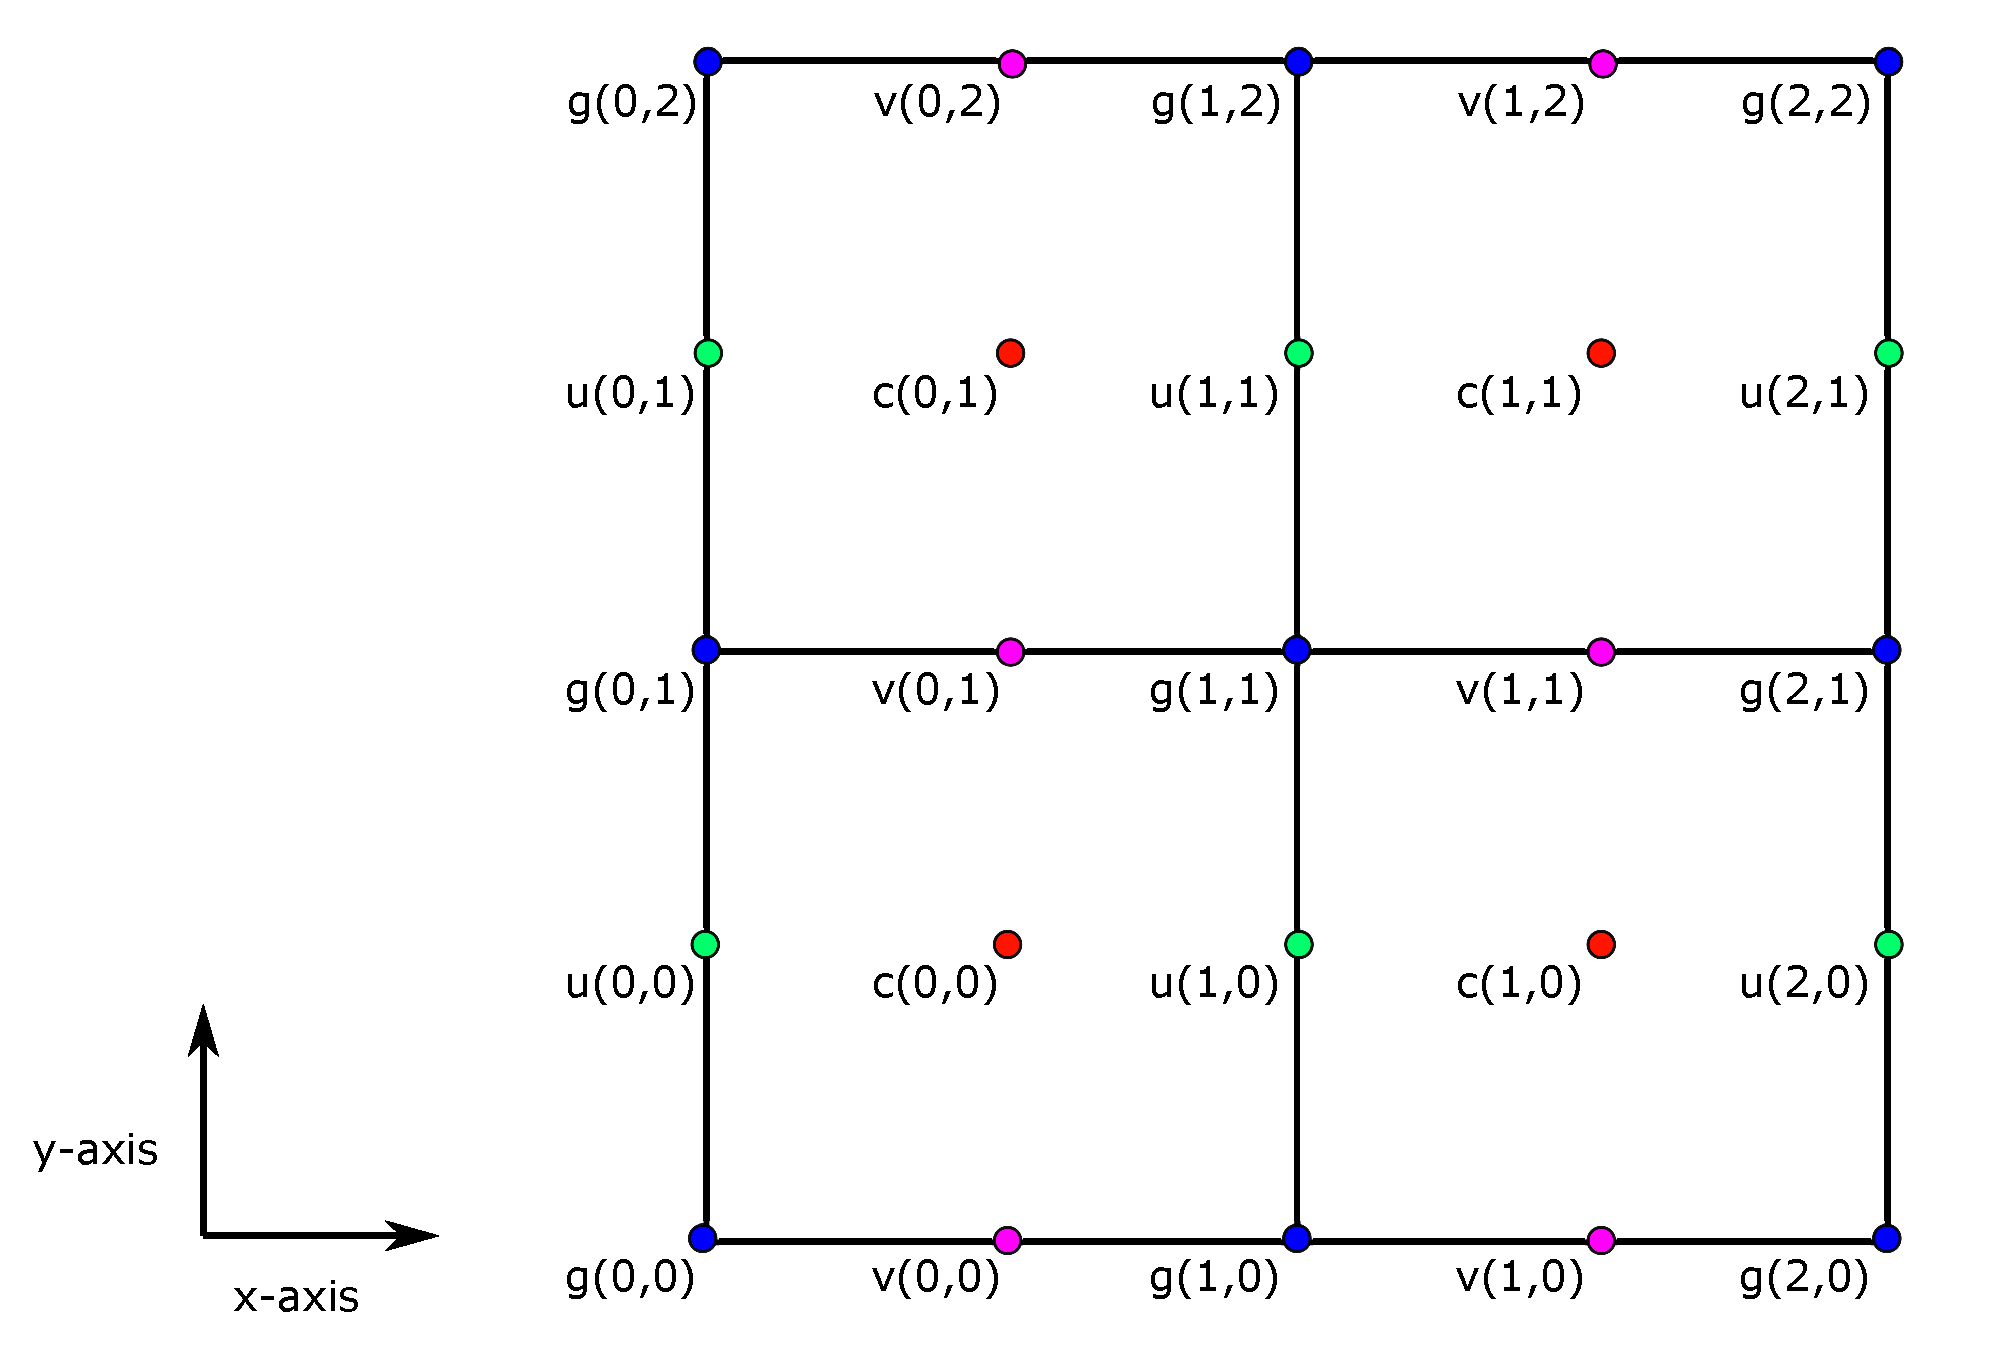
\includegraphics{../figures/C-grid-points.png} \textbf{The four
different categories of point used in the staggered Arakawa-C grid
(C-grid)}

\subsubsection{\texorpdfstring{\emph{c}
points}{c points}}\label{c-points}

Scalar variables (e.g., \(T, S, SSH, OBP, SIarea\)) and variables
associated with vertical velocity (e.g., \(WVEL\)) are situated at the
center of the tracer grid cell in the horizontal plane. These are \(c\)
points

Define the coordinates \((i,j)\) for the discrete indices of \(c\)
points in the \(x\) and \(y\) directions, respectively.

In the ECCO v4 NetCDF files, \(c(0,0)\) is the \(-x\) most and \(-y\)
most tracer grid cell.

\begin{itemize}
\tightlist
\item
  In the +\(y\) direction, the next \(c\) point is \(c(0,1)\).
\item
  In the +\(x\) direction, the next \(c\) point is \(c(1,0)\)
\end{itemize}

\subsubsection{\texorpdfstring{\emph{u}
points}{u points}}\label{u-points}

Vector variables related to horizontal velocity in the \(x\) direction
are staggered along the edges of tracer cells between \(c\) points in
the horizontal plane. Examples include horizontal velocity in the \(x\)
direction (\(UVEL\)) and horizontal advective flux of snow in the \(x\)
direction (\(ADVxSNOW\)). They are situated along the edges (if 2D) or
faces (if 3D) of the tracer grid cells in the \(x\) direction.

Define the coordinates \((i_g,j)\) for the discrete indices of \(u\)
points in the \(x\) and \(y\) directions, respectively.

We use \(i_g\) as the coordinate in the \(x\) direction because \(u\)
points are situated along the tracer grid cell ed\textbf{\emph{G}}es. We
use \(j\) for its \(y\) coordinate because \(u\) points and \(c\) points
fall along the same lines in \(y\).

In the ECCO v4 netCDF files, \(u(0,0)\) is the \(-x\) most and \(-y\)
most \(u\) point.

\subsubsection{\texorpdfstring{\emph{v}
points}{v points}}\label{v-points}

Vector variables related to horizontal velocity in the \(y\) direction
are staggered along the edges of tracer cells between \(c\) points in
the horizontal plane. Examples include horizontal velocity in the \(y\)
direction (\(VVEL\)) and horizontal advective flux of snow in the \(y\)
direction (\(ADVySNOW\)). They are situated along the edges (if 2D) or
faces (if 3D) of the tracer grid cells in the \(y\) direction.

Define the coordinates \((i,j_g)\) for the discrete indices of \(v\)
points in the \(x\) and \(y\) directions, respectively.

We use \(j_g\) as the coordinate in the \(y\) direction because \(v\)
points are situated along the tracer grid cell ed\textbf{\emph{G}}es. We
use \(i\) for its \(x\) coordinate because \(v\) points and \(c\) points
fall along the same lines in \(x\).

In the ECCO v4 NetCDF files, \(v(0,0)\) is the \(-x\) most and \(-y\)
most \(v\) point.

\subsubsection{\texorpdfstring{\emph{g}
points}{g points}}\label{g-points}

Variables that are explictly related to horizontal velocities in the
model in both the \(x\) and \(y\) direction are situated at \(g\) points
in the horizontal plane. \(g\) points are situated at the corners of
tracer grid cells.

Define the coordinates \((i_g,j_g)\) for the discrete indices of \(g\)
points in the \(x\) and \(y\) directions, respectively.

We use \(i_g\) and \(j_g\) because \(g\) points are on the
ed\textbf{\emph{G}}es (corners) of tracer grid cells.

In the ECCO v4 NetCDF files, \(g(0,0)\) is the \(-x\) most and \(-y\)
most \(g\) point.

\subsection{The two vertical points of the
c-grid}\label{the-two-vertical-points-of-the-c-grid}

There are two different coordinates in the vertical \(z\) dimension:

\subsubsection{\texorpdfstring{\emph{w}
points}{w points}}\label{w-points}

Variables related to vertical velocity or vertical fluxes are situated
at \(w\) points in the vertical direction. These variables are situated
on the upper and lower faces of the tracer grid cell.

Define the coordinate \(k_g\) for \(w\) points using the same reasoning
as above: \(w\) points fall along the the ed\textbf{\emph{G}}es of
tracer grid cells in the \(z\) direction (top and bottom of the grid
cells).

In the ECCO v4 NetCDF files, \(k_g(0)\) is the sea surface.

\subsubsection{\texorpdfstring{\emph{k}
points}{k points}}\label{k-points}

Variables that are not related to vertical velocity or vertical fluxes
are situated at \(k\) points in the vertical direction. These variables
are situated on the upper and lower faces of the tracer grid cell.

Define the coordinate \(k\) for points situated in the center of the
grid cells.

In the ECCO v4 NetCDF files, \(k(0)\) is the middle of the uppermost
tracer grid cell.

\subsection{Applying the C-grid coordinates to the
variables}\label{applying-the-c-grid-coordinates-to-the-variables}

The default coordinate names in the ECCO v4 netcdf tile files do not
distinguish distinguish between the four horizontal coordinates,
\(i, i_g, j, j_g\) and the two vertical coordinates, \(k_g\) and \(k\),
used by our c-grid model.

To apply these more descriptive coordinates to the \texttt{Dataset}
objects that are created when we load netCDF files, we provide a special
routine, \texttt{load\_tile\_from\_netcdf}.

\subsubsection{\texorpdfstring{\texttt{load\_tile\_from\_netcdf}}{load\_tile\_from\_netcdf}}\label{load_tile_from_netcdf}

This routine takes four arguments, 1. \emph{data\_dir}: the directory of
the netCDF file 2. \emph{var}: the name of the variable stored in the
netCDF file (without the tile number). Examples include \emph{THETA},
\emph{VVEL}, \emph{DFxEHFF} 3. \emph{var\_type}: one of 'c','g','u','v',
or 'grid' corresponding with the variable's c-grid point type. 'grid' is
a special case because unlike every other variable NetCDF file, grid
files actually contain several variables that are on different c-grid
points. 4. \emph{tile\_index}: the tile number {[}1 .. 13{]}

    \subsubsection{\texorpdfstring{Loading an ECCO v4 netCDF grid tile file
using
\texttt{load\_tile\_from\_netcdf}}{Loading an ECCO v4 netCDF grid tile file using load\_tile\_from\_netcdf}}\label{loading-an-ecco-v4-netcdf-grid-tile-file-using-load_tile_from_netcdf}

Let's use \texttt{load\_tile\_from\_netcdf} to load grid tile 3 again.
This time we'll call the new \texttt{Dataset} object
\texttt{grid\_3\_new}

    \begin{Verbatim}[commandchars=\\\{\}]
{\color{incolor}In [{\color{incolor}71}]:} \PY{n}{var} \PY{o}{=} \PY{l+s+s1}{\PYZsq{}}\PY{l+s+s1}{GRID}\PY{l+s+s1}{\PYZsq{}}
         \PY{n}{var\PYZus{}type} \PY{o}{=} \PY{l+s+s1}{\PYZsq{}}\PY{l+s+s1}{grid}\PY{l+s+s1}{\PYZsq{}}
         \PY{n}{tile\PYZus{}index} \PY{o}{=} \PY{l+m+mi}{3}
         \PY{n}{grid\PYZus{}3\PYZus{}new} \PY{o}{=} \PY{n}{ecco}\PY{o}{.}\PY{n}{load\PYZus{}tile\PYZus{}from\PYZus{}netcdf}\PY{p}{(}\PY{n}{grid\PYZus{}dir}\PY{p}{,} \PY{n}{var}\PY{p}{,} \PY{n}{var\PYZus{}type}\PY{p}{,} \PY{n}{tile\PYZus{}index}\PY{p}{)}
\end{Verbatim}


    \begin{Verbatim}[commandchars=\\\{\}]
loading /Volumes/ECCO\_BASE/ECCO\_v4r3/nctiles\_grid/GRID.0003.nc

    \end{Verbatim}

    \begin{Verbatim}[commandchars=\\\{\}]
{\color{incolor}In [{\color{incolor}72}]:} \PY{n}{grid\PYZus{}3\PYZus{}new}
\end{Verbatim}


\begin{Verbatim}[commandchars=\\\{\}]
{\color{outcolor}Out[{\color{outcolor}72}]:} <xarray.Dataset>
         Dimensions:  (i: 90, i\_g: 90, j: 90, j\_g: 90, k: 50, k\_g: 50)
         Coordinates:
             tile     int64 3
           * k        (k) float64 1.0 2.0 3.0 4.0 5.0 6.0 7.0 8.0 9.0 10.0 11.0 12.0 {\ldots}
           * i        (i) float64 1.0 2.0 3.0 4.0 5.0 6.0 7.0 8.0 9.0 10.0 11.0 12.0 {\ldots}
           * j        (j) float64 1.0 2.0 3.0 4.0 5.0 6.0 7.0 8.0 9.0 10.0 11.0 12.0 {\ldots}
           * i\_g      (i\_g) float64 1.0 2.0 3.0 4.0 5.0 6.0 7.0 8.0 9.0 10.0 11.0 {\ldots}
           * j\_g      (j\_g) float64 1.0 2.0 3.0 4.0 5.0 6.0 7.0 8.0 9.0 10.0 11.0 {\ldots}
           * k\_g      (k\_g) float64 1.0 2.0 3.0 4.0 5.0 6.0 7.0 8.0 9.0 10.0 11.0 {\ldots}
         Data variables:
             XC       (j, i) float64 {\ldots}
             YC       (j, i) float64 {\ldots}
             RAC      (j, i) float64 {\ldots}
             Depth    (j, i) float64 {\ldots}
             AngleCS  (j, i) float64 {\ldots}
             AngleSN  (j, i) float64 {\ldots}
             hFacC    (k, j, i) float64 {\ldots}
             land\_c   (k, j, i) float64 1.0 1.0 1.0 1.0 1.0 1.0 1.0 1.0 1.0 1.0 1.0 {\ldots}
             XG       (j\_g, i\_g) float64 {\ldots}
             YG       (j\_g, i\_g) float64 {\ldots}
             RAZ      (j\_g, i\_g) float64 {\ldots}
             DXC      (j, i\_g) float64 {\ldots}
             DYG      (j, i\_g) float64 {\ldots}
             hFacW    (k, j, i\_g) float64 {\ldots}
             land\_u   (k, j, i\_g) float64 1.0 1.0 1.0 1.0 1.0 1.0 1.0 1.0 1.0 1.0 1.0 {\ldots}
             DYC      (j\_g, i) float64 {\ldots}
             DXG      (j\_g, i) float64 {\ldots}
             hFacS    (k, j\_g, i) float64 {\ldots}
             land\_v   (k, j\_g, i) float64 1.0 1.0 1.0 1.0 1.0 1.0 1.0 1.0 1.0 1.0 1.0 {\ldots}
             RF       (k\_g) float64 {\ldots}
             DRC      (k\_g) float64 {\ldots}
             RC       (k) float64 {\ldots}
             DRF      (k) float64 {\ldots}
         Attributes:
             description:    C-grid parameters (see MITgcm documentation for details){\ldots}
             A:              :Format      = native grid (nctiles w. 13 tiles)
             B:              :source      = ECCO consortium (http://ecco-group.org/)
             C:              :institution = JPL/UT/MIT/AER
             D:              :history     = files revision history :
             E:                                 04/20/2017: fill in geometry info for {\ldots}
             F:                                 11/06/2016: third release of ECCO v4 ({\ldots}
             G:                             estimates revision history (from second re{\ldots}
             H:                                 employs bi-harmonic viscosity (enhance{\ldots}
             I:                                 sea-ice parameters, updated or novel o{\ldots}
             J:                                 GRACE OBP, Aquarius SSS, global mean s{\ldots}
             K:                                 time-series, extended and/or expanded {\ldots}
             L:                                 revised weights including data and con{\ldots}
             M:                                 to account for grid-size variation and{\ldots}
             N:                                 separate time-mean and time-variable d{\ldots}
             O:                                 and controls, sea-ice costs, and initi{\ldots}
             P:                                 additional controls.\textbackslash{}n 
             Q:              :references  = Forget, G., J.-M. Campin, P. Heimbach, C. {\ldots}
             R:                              and C. Wunsch, 2015: ECCO version 4: an i{\ldots}
             S:                              non-linear inverse modeling and global oc{\ldots}
             T:                              Geoscientific Model Development, 8, 3071-{\ldots}
             U:                             Forget, G., J.-M. Campin, P. Heimbach, C. {\ldots}
             V:                              ECCO version 4: Second Release, 2016, htt{\ldots}
             W:              file created using gcmfaces\_IO/write2nctiles.m
             date:           21-Apr-2017
             Conventions:    CF-1.6
             \_FillValue:     nan
             missing\_value:  nan
\end{Verbatim}
            
    \subsubsection{Examining the Dataset object
contents}\label{examining-the-dataset-object-contents}

\paragraph{1. Dimensions}\label{dimensions}

\texttt{Dimensions:\ \ (i:\ 90,\ i\_g:\ 90,\ j:\ 90,\ j\_g:\ 90,\ k:\ 50,\ k\_g:\ 50)}

The \emph{Dimensions} list now lists the six different coordinates and
their dimension used by variables stored in this new grid tile
\texttt{Dataset} object.

\paragraph{2. Coordinates}\label{coordinates}

\begin{verbatim}
Coordinates:
    tile     int64 3
  * k        (k) float64 1.0 2.0 3.0 4.0 5.0 6.0 7.0 8.0 9.0 10.0 11.0 12.0 ...
  * i        (i) float64 1.0 2.0 3.0 4.0 5.0 6.0 7.0 8.0 9.0 10.0 11.0 12.0 ...
  * j        (j) float64 1.0 2.0 3.0 4.0 5.0 6.0 7.0 8.0 9.0 10.0 11.0 12.0 ...
  * i_g      (i_g) float64 1.0 2.0 3.0 4.0 5.0 6.0 7.0 8.0 9.0 10.0 11.0 ...
  * j_g      (j_g) float64 1.0 2.0 3.0 4.0 5.0 6.0 7.0 8.0 9.0 10.0 11.0 ...
  * k_g      (k_g) float64 1.0 2.0 3.0 4.0 5.0 6.0 7.0 8.0 9.0 10.0 11.0 ...
\end{verbatim}

Each of the 6 dimensions has a corresponding set of coordinate labels.

\paragraph{3. Data Variables}\label{data-variables}

\begin{verbatim}
Data variables:
    XC       (j, i) float64 ...
    hFacC    (k, j, i) float64 ...
    XG       (j_g, i_g) float64 ...
    DXC      (j, i_g) float64 ...
    hFacW    (k, j, i_g) float64 ...
    DYC      (j_g, i) float64 ...
    hFacS    (k, j_g, i) float64 ...
    RF       (k_g) float64 ...
    RC       (k) float64 ...
\end{verbatim}

We now see that each \emph{data variable} is now described with its
proper coordinates. For example, XC, the longitude of the tracer grid
cell center uses \(i,j\) coordiantes while XG, the longitude grid cell
corners, now has \(i_g, j_g\) coordinates. DXC, the distance between
adjacent cell centers, uses \(i_g, j\) coordiantes: consistent with the
notion that distances between cell centers in \(x\) are situated halfway
between cell centers.

\begin{quote}
\textbf{Note:} The ordering of arrays is not (x,y,z) but (z,y,x).
\end{quote}

In addition to the variables now having more descriptive coordinates,
the \texttt{load\_tile\_from\_netcdf} routine also adds 3 new
three-dimensional land masks, one each for grid cell at the 'u'
(land\_u), 'c' (land\_c), and 'v' (land\_v) points.

    \subsection{\texorpdfstring{A closer look at the DataArray after loading
with
\texttt{load\_tile\_from\_netcdf}}{A closer look at the DataArray after loading with load\_tile\_from\_netcdf}}\label{a-closer-look-at-the-dataarray-after-loading-with-load_tile_from_netcdf}

Let's take a quick look at one of the variables loaded using the
\texttt{load\_tile\_from\_netcdf} routine:

    \begin{Verbatim}[commandchars=\\\{\}]
{\color{incolor}In [{\color{incolor}73}]:} \PY{n}{grid\PYZus{}3\PYZus{}new}\PY{o}{.}\PY{n}{XC}
\end{Verbatim}


\begin{Verbatim}[commandchars=\\\{\}]
{\color{outcolor}Out[{\color{outcolor}73}]:} <xarray.DataArray 'XC' (j: 90, i: 90)>
         array([[-37.5     , -36.5     , -35.5     , {\ldots},  49.5     ,  50.5     ,  51.5     ],
                [-37.5     , -36.5     , -35.5     , {\ldots},  49.5     ,  50.5     ,  51.5     ],
                [-37.5     , -36.5     , -35.5     , {\ldots},  49.5     ,  50.5     ,  51.5     ],
                {\ldots}, 
                [-37.730072, -37.178291, -36.597565, {\ldots},  50.597565,  51.178291,
                  51.730072],
                [-37.771988, -37.291943, -36.764027, {\ldots},  50.764027,  51.291943,
                  51.771988],
                [-37.837925, -37.44421 , -36.968143, {\ldots},  50.968143,  51.44421 ,
                  51.837925]])
         Coordinates:
             tile     int64 3
           * i        (i) float64 1.0 2.0 3.0 4.0 5.0 6.0 7.0 8.0 9.0 10.0 11.0 12.0 {\ldots}
           * j        (j) float64 1.0 2.0 3.0 4.0 5.0 6.0 7.0 8.0 9.0 10.0 11.0 12.0 {\ldots}
         Attributes:
             long\_name:          longitude
             units:              degrees\_east
             rotated\_to\_latlon:  False
\end{Verbatim}
            
    The \texttt{load\_tile\_from\_netcdf} routine adds a new coordinate to
the variables, \emph{tile}. This will be helpful when loading and
combining multiple tiles.

Finally, we see a new attribute: \emph{rotated\_to\_latlon}. This
attribute is a flag telling us that the arrays are in the original
lat-lon-cap tile layout. We'll discuss this later.

    \subsection{\texorpdfstring{Loading non-grid ECCO variables using
\texttt{load\_tile\_from\_netcdf}}{Loading non-grid ECCO variables using load\_tile\_from\_netcdf}}\label{loading-non-grid-ecco-variables-using-load_tile_from_netcdf}

So far we've only looked at ECCO v4 grid tile files. With the
\texttt{load\_tile\_from\_netcdf} routine you can assign the proper
coordinates to any variable by specifying its c-grid point category.

We'll demonstrate by loading three variables, one each that are on
'c','u', and 'v' points

\subsubsection{A 'c' point variable: SSH}\label{a-c-point-variable-ssh}

Let's load tile 3 of the 'c' point sea surface height (SSH) variable.

    \begin{Verbatim}[commandchars=\\\{\}]
{\color{incolor}In [{\color{incolor}74}]:} \PY{n}{data\PYZus{}dir}\PY{o}{=}\PY{l+s+s1}{\PYZsq{}}\PY{l+s+s1}{/Volumes/ECCO\PYZus{}BASE/ECCO\PYZus{}v4r3/nctiles\PYZus{}monthly/SSH/}\PY{l+s+s1}{\PYZsq{}}    
         \PY{n}{var} \PY{o}{=} \PY{l+s+s1}{\PYZsq{}}\PY{l+s+s1}{SSH}\PY{l+s+s1}{\PYZsq{}}
         \PY{n}{var\PYZus{}type} \PY{o}{=} \PY{l+s+s1}{\PYZsq{}}\PY{l+s+s1}{c}\PY{l+s+s1}{\PYZsq{}}
         \PY{n}{tile\PYZus{}index} \PY{o}{=} \PY{l+m+mi}{3}
         \PY{n}{ssh\PYZus{}tile\PYZus{}3} \PY{o}{=} \PY{n}{ecco}\PY{o}{.}\PY{n}{load\PYZus{}tile\PYZus{}from\PYZus{}netcdf}\PY{p}{(}\PY{n}{data\PYZus{}dir}\PY{p}{,} \PY{n}{var}\PY{p}{,} \PY{n}{var\PYZus{}type}\PY{p}{,} \PY{n}{tile\PYZus{}index}\PY{p}{)}
\end{Verbatim}


    \begin{Verbatim}[commandchars=\\\{\}]
loading /Volumes/ECCO\_BASE/ECCO\_v4r3/nctiles\_monthly/SSH/SSH.0003.nc

    \end{Verbatim}

    Since this is the first time we're loading an output variable from the
state estimate let's closely examine \texttt{ssh\_tile\_3}.

    \begin{Verbatim}[commandchars=\\\{\}]
{\color{incolor}In [{\color{incolor}75}]:} \PY{n}{ssh\PYZus{}tile\PYZus{}3}
\end{Verbatim}


\begin{Verbatim}[commandchars=\\\{\}]
{\color{outcolor}Out[{\color{outcolor}75}]:} <xarray.Dataset>
         Dimensions:   (i: 90, j: 90, tile: 1, time: 288)
         Coordinates:
           * time      (time) float64 1.0 2.0 3.0 4.0 5.0 6.0 7.0 8.0 9.0 10.0 11.0 {\ldots}
           * j         (j) float64 1.0 2.0 3.0 4.0 5.0 6.0 7.0 8.0 9.0 10.0 11.0 12.0 {\ldots}
           * i         (i) float64 1.0 2.0 3.0 4.0 5.0 6.0 7.0 8.0 9.0 10.0 11.0 12.0 {\ldots}
             lon\_c     (j, i) float64 -37.5 -36.5 -35.5 -34.5 -33.5 -32.5 -31.5 -30.5 {\ldots}
             lat\_c     (j, i) float64 10.46 10.46 10.46 10.46 10.46 10.46 10.46 10.46 {\ldots}
             tim       (time) datetime64[ns] {\ldots}
           * tile      (tile) int64 3
             timestep  (time) float64 732.0 1.428e+03 2.172e+03 2.892e+03 3.636e+03 {\ldots}
         Data variables:
             SSH       (time, tile, j, i) float64 0.0576 0.05474 0.05277 0.05157 {\ldots}
         Attributes:
             description:    SSH -- ECCO v4 ocean state estimate, release 3 -- 1992-2015
             A:              :Format      = native grid (nctiles w. 13 tiles)
             B:              :source      = ECCO consortium (http://ecco-group.org/)
             C:              :institution = JPL/UT/MIT/AER
             D:              :history     = files revision history :
             E:                                 05/02/2017: adjust SSH and OBP with gl{\ldots}
             F:                                 05/02/2017: adjust SSH with sea-ice lo{\ldots}
             G:                                 04/20/2017: fill in geometry info for {\ldots}
             H:                                 11/06/2016: third release of ECCO v4 ({\ldots}
             I:                             estimates revision history (from second re{\ldots}
             J:                                 employs bi-harmonic viscosity (enhance{\ldots}
             K:                                 sea-ice parameters, updated or novel o{\ldots}
             L:                                 GRACE OBP, Aquarius SSS, global mean s{\ldots}
             M:                                 time-series, extended and/or expanded {\ldots}
             N:                                 revised weights including data and con{\ldots}
             O:                                 to account for grid-size variation and{\ldots}
             P:                                 separate time-mean and time-variable d{\ldots}
             Q:                                 and controls, sea-ice costs, and initi{\ldots}
             R:                                 additional controls.\textbackslash{}n 
             S:              :references  = Forget, G., J.-M. Campin, P. Heimbach, C. {\ldots}
             T:                              and C. Wunsch, 2015: ECCO version 4: an i{\ldots}
             U:                              non-linear inverse modeling and global oc{\ldots}
             V:                              Geoscientific Model Development, 8, 3071-{\ldots}
             W:                             Forget, G., J.-M. Campin, P. Heimbach, C. {\ldots}
             X:                              ECCO version 4: Second Release, 2016, htt{\ldots}
             Y:              file created using gcmfaces\_IO/write2nctiles.m
             date:           02-May-2017
             Conventions:    CF-1.6
             \_FillValue:     nan
             missing\_value:  nan
\end{Verbatim}
            
    Notice that unlike the grid files that we've loaded up until now, the
\texttt{ssh\_tile\_3} \texttt{Dataset} object only has one \emph{Data
variable}, \(SSH\). Non-grid ECCO v4 NetCDF tile files only ever store
\emph{one} physical variable. Consequently, the \emph{dimensions} of the
\texttt{Dataset} will be the same as the \emph{dimensions} of the single
\emph{data variable}. Let's take a look at the \(SSH\)
\texttt{DataArary}:

    \begin{Verbatim}[commandchars=\\\{\}]
{\color{incolor}In [{\color{incolor}76}]:} \PY{n}{ssh\PYZus{}tile\PYZus{}3}\PY{o}{.}\PY{n}{SSH}
\end{Verbatim}


\begin{Verbatim}[commandchars=\\\{\}]
{\color{outcolor}Out[{\color{outcolor}76}]:} <xarray.DataArray 'SSH' (time: 288, tile: 1, j: 90, i: 90)>
         array([[[[ 0.0576  , {\ldots},  0.383994],
                  {\ldots}, 
                  [      nan, {\ldots},       nan]]],
         
         
                {\ldots}, 
                [[[ 0.075663, {\ldots},  0.458817],
                  {\ldots}, 
                  [      nan, {\ldots},       nan]]]])
         Coordinates:
           * time      (time) float64 1.0 2.0 3.0 4.0 5.0 6.0 7.0 8.0 9.0 10.0 11.0 {\ldots}
           * j         (j) float64 1.0 2.0 3.0 4.0 5.0 6.0 7.0 8.0 9.0 10.0 11.0 12.0 {\ldots}
           * i         (i) float64 1.0 2.0 3.0 4.0 5.0 6.0 7.0 8.0 9.0 10.0 11.0 12.0 {\ldots}
             lon\_c     (j, i) float64 -37.5 -36.5 -35.5 -34.5 -33.5 -32.5 -31.5 -30.5 {\ldots}
             lat\_c     (j, i) float64 10.46 10.46 10.46 10.46 10.46 10.46 10.46 10.46 {\ldots}
             tim       (time) datetime64[ns] {\ldots}
           * tile      (tile) int64 3
             timestep  (time) float64 732.0 1.428e+03 2.172e+03 2.892e+03 3.636e+03 {\ldots}
         Attributes:
             long\_name:          Surface Height Anomaly adjusted with global steric he{\ldots}
             units:              m
             rotated\_to\_latlon:  False
\end{Verbatim}
            
    \paragraph{Dimensional coordinates}\label{dimensional-coordinates}

As expected, the \texttt{SSH} \texttt{DataArray} uses \textbf{i, j}
coordinates for its horizontal dimensions. We also see a \textbf{tile}
and \textbf{time} coordinates. The ordering of the \(SSH\) dimensions is
\textbf{time, tile, j, i} with the logic being that \textbf{tile} is a
kind of space coordinate.

We find 288 records in the \textbf{time} dimensions. One for each month
of the 1992-2015 state estimate. There is one record in the
\textbf{tile} dimensions because we have only loaded a single tile file
so far.

\paragraph{Non-dimensional
coordinates}\label{non-dimensional-coordinates}

Notice the four \emph{Coordinates} that do not have an "*" in front of
their names. These are so-called
\href{http://xarray.pydata.org/en/stable/data-structures.html\#coordinates}{non-dimensional
coordinates}. Think of non-dimensional coordinates as helpful extra
coordinate labels. Here, the non-dimensional coordinates include two for
the \textbf{time} dimension: \textbf{tim} and \textbf{timestep}, and two
for the space dimensions: \textbf{lon\_c, lat\_c}.

\subparagraph{The time non-dimensional
coordinates}\label{the-time-non-dimensional-coordinates}

    \begin{Verbatim}[commandchars=\\\{\}]
{\color{incolor}In [{\color{incolor}77}]:} \PY{n}{ssh\PYZus{}tile\PYZus{}3}\PY{o}{.}\PY{n}{time}
\end{Verbatim}


\begin{Verbatim}[commandchars=\\\{\}]
{\color{outcolor}Out[{\color{outcolor}77}]:} <xarray.DataArray 'time' (time: 288)>
         array([   1.,    2.,    3., {\ldots},  286.,  287.,  288.])
         Coordinates:
           * time      (time) float64 1.0 2.0 3.0 4.0 5.0 6.0 7.0 8.0 9.0 10.0 11.0 {\ldots}
             tim       (time) datetime64[ns] {\ldots}
             timestep  (time) float64 732.0 1.428e+03 2.172e+03 2.892e+03 3.636e+03 {\ldots}
         Attributes:
             long\_name:  array index 1
             units:      1
\end{Verbatim}
            
    The \textbf{tim} non-dimensional coordinate provides the calendar date
(centered in the month) for the \textbf{time} monthly index and the
\textbf{timestep} non-dimensional coordinate provides the the timestep
number corresponding to each month (the ECCO v4 simulation uses 1-hourly
timesteps).

\subparagraph{The space non-dimensional
coordinates}\label{the-space-non-dimensional-coordinates}

\textbf{lon\_c} and \textbf{lat\_c} non-dimensional coordinates provide
the longitude and latitude for each of the 'c' points of \(SSH\).

    \begin{Verbatim}[commandchars=\\\{\}]
{\color{incolor}In [{\color{incolor}78}]:} \PY{n}{ssh\PYZus{}tile\PYZus{}3}\PY{o}{.}\PY{n}{lon\PYZus{}c}
\end{Verbatim}


\begin{Verbatim}[commandchars=\\\{\}]
{\color{outcolor}Out[{\color{outcolor}78}]:} <xarray.DataArray 'lon\_c' (j: 90, i: 90)>
         array([[-37.5     , -36.5     , -35.5     , {\ldots},  49.5     ,  50.5     ,  51.5     ],
                [-37.5     , -36.5     , -35.5     , {\ldots},  49.5     ,  50.5     ,  51.5     ],
                [-37.5     , -36.5     , -35.5     , {\ldots},  49.5     ,  50.5     ,  51.5     ],
                {\ldots}, 
                [-37.730072, -37.178291, -36.597565, {\ldots},  50.597565,  51.178291,
                  51.730072],
                [-37.771988, -37.291943, -36.764027, {\ldots},  50.764027,  51.291943,
                  51.771988],
                [-37.837925, -37.44421 , -36.968143, {\ldots},  50.968143,  51.44421 ,
                  51.837925]])
         Coordinates:
           * j        (j) float64 1.0 2.0 3.0 4.0 5.0 6.0 7.0 8.0 9.0 10.0 11.0 12.0 {\ldots}
           * i        (i) float64 1.0 2.0 3.0 4.0 5.0 6.0 7.0 8.0 9.0 10.0 11.0 12.0 {\ldots}
             lon\_c    (j, i) float64 -37.5 -36.5 -35.5 -34.5 -33.5 -32.5 -31.5 -30.5 {\ldots}
             lat\_c    (j, i) float64 10.46 10.46 10.46 10.46 10.46 10.46 10.46 10.46 {\ldots}
         Attributes:
             units:          degrees\_east
             standard\_name:  longitude
\end{Verbatim}
            
    \subsubsection{A 'u' point variable:
UVEL}\label{a-u-point-variable-uvel}

Let's load tile 3 of the 'u' point horizontal velocity in the local
\(x\) direction variable, \(UVEL\).

    \begin{Verbatim}[commandchars=\\\{\}]
{\color{incolor}In [{\color{incolor}79}]:} \PY{n}{data\PYZus{}dir}\PY{o}{=}\PY{l+s+s1}{\PYZsq{}}\PY{l+s+s1}{/Volumes/ECCO\PYZus{}BASE/ECCO\PYZus{}v4r3/nctiles\PYZus{}monthly/UVEL/}\PY{l+s+s1}{\PYZsq{}}    
         \PY{n}{var} \PY{o}{=} \PY{l+s+s1}{\PYZsq{}}\PY{l+s+s1}{UVEL}\PY{l+s+s1}{\PYZsq{}}
         \PY{n}{var\PYZus{}type} \PY{o}{=} \PY{l+s+s1}{\PYZsq{}}\PY{l+s+s1}{u}\PY{l+s+s1}{\PYZsq{}}
         \PY{n}{tile\PYZus{}index} \PY{o}{=} \PY{l+m+mi}{3}
         \PY{n}{uvel\PYZus{}tile\PYZus{}3} \PY{o}{=} \PY{n}{ecco}\PY{o}{.}\PY{n}{load\PYZus{}tile\PYZus{}from\PYZus{}netcdf}\PY{p}{(}\PY{n}{data\PYZus{}dir}\PY{p}{,} \PY{n}{var}\PY{p}{,} \PY{n}{var\PYZus{}type}\PY{p}{,} \PY{n}{tile\PYZus{}index}\PY{p}{)}
\end{Verbatim}


    \begin{Verbatim}[commandchars=\\\{\}]
loading /Volumes/ECCO\_BASE/ECCO\_v4r3/nctiles\_monthly/UVEL/UVEL.0003.nc

    \end{Verbatim}

    Let's look at \texttt{uvel\_tile\_3}. This time let's also remove some
of the descriptive NetCDF file \emph{Attributes} using a little routine
called \texttt{minimal\_metadata}. We've already seen these attributes a
number of times.

    \begin{Verbatim}[commandchars=\\\{\}]
{\color{incolor}In [{\color{incolor}80}]:} \PY{n}{ecco}\PY{o}{.}\PY{n}{minimal\PYZus{}metadata}\PY{p}{(}\PY{n}{uvel\PYZus{}tile\PYZus{}3}\PY{p}{)}
\end{Verbatim}


    \begin{Verbatim}[commandchars=\\\{\}]
Removing Dataset Attributes A-Z


    \end{Verbatim}

    \begin{Verbatim}[commandchars=\\\{\}]
{\color{incolor}In [{\color{incolor}81}]:} \PY{n}{uvel\PYZus{}tile\PYZus{}3}
\end{Verbatim}


\begin{Verbatim}[commandchars=\\\{\}]
{\color{outcolor}Out[{\color{outcolor}81}]:} <xarray.Dataset>
         Dimensions:   (i\_g: 90, j: 90, k: 50, tile: 1, time: 288)
         Coordinates:
           * time      (time) float64 1.0 2.0 3.0 4.0 5.0 6.0 7.0 8.0 9.0 10.0 11.0 {\ldots}
           * k         (k) float64 1.0 2.0 3.0 4.0 5.0 6.0 7.0 8.0 9.0 10.0 11.0 12.0 {\ldots}
           * j         (j) float64 1.0 2.0 3.0 4.0 5.0 6.0 7.0 8.0 9.0 10.0 11.0 12.0 {\ldots}
           * i\_g       (i\_g) float64 1.0 2.0 3.0 4.0 5.0 6.0 7.0 8.0 9.0 10.0 11.0 {\ldots}
             lon\_u     (j, i\_g) float64 -38.0 -37.0 -36.0 -35.0 -34.0 -33.0 -32.0 {\ldots}
             lat\_u     (j, i\_g) float64 10.46 10.46 10.46 10.46 10.46 10.46 10.46 {\ldots}
             dep       (k) float64 {\ldots}
             tim       (time) datetime64[ns] {\ldots}
           * tile      (tile) int64 3
             timestep  (time) float64 732.0 1.428e+03 2.172e+03 2.892e+03 3.636e+03 {\ldots}
         Data variables:
             UVEL      (time, tile, k, j, i\_g) float64 -0.02911 -0.02432 -0.02008 {\ldots}
         Attributes:
             description:    UVEL -- ECCO v4 ocean state estimate, release 3 -- 1992-2015
             date:           03-Nov-2017
             Conventions:    CF-1.6
             \_FillValue:     nan
             missing\_value:  nan
\end{Verbatim}
            
    \texttt{uvel\_tile\_3} has one \emph{Data variable}, \(UVEL\). Let's
take a look at the \(UVEL\) \texttt{DataArary}:

    \begin{Verbatim}[commandchars=\\\{\}]
{\color{incolor}In [{\color{incolor}82}]:} \PY{n}{uvel\PYZus{}tile\PYZus{}3}\PY{o}{.}\PY{n}{UVEL}
\end{Verbatim}


\begin{Verbatim}[commandchars=\\\{\}]
{\color{outcolor}Out[{\color{outcolor}82}]:} <xarray.DataArray 'UVEL' (time: 288, tile: 1, k: 50, j: 90, i\_g: 90)>
         array([[[[[-0.029109, {\ldots},       nan],
                   {\ldots}, 
                   [      nan, {\ldots},       nan]],
         
                  {\ldots}, 
                  [[      nan, {\ldots},       nan],
                   {\ldots}, 
                   [      nan, {\ldots},       nan]]]],
         
         
         
                {\ldots}, 
                [[[[-0.050949, {\ldots},       nan],
                   {\ldots}, 
                   [      nan, {\ldots},       nan]],
         
                  {\ldots}, 
                  [[      nan, {\ldots},       nan],
                   {\ldots}, 
                   [      nan, {\ldots},       nan]]]]])
         Coordinates:
           * time      (time) float64 1.0 2.0 3.0 4.0 5.0 6.0 7.0 8.0 9.0 10.0 11.0 {\ldots}
           * k         (k) float64 1.0 2.0 3.0 4.0 5.0 6.0 7.0 8.0 9.0 10.0 11.0 12.0 {\ldots}
           * j         (j) float64 1.0 2.0 3.0 4.0 5.0 6.0 7.0 8.0 9.0 10.0 11.0 12.0 {\ldots}
           * i\_g       (i\_g) float64 1.0 2.0 3.0 4.0 5.0 6.0 7.0 8.0 9.0 10.0 11.0 {\ldots}
             lon\_u     (j, i\_g) float64 -38.0 -37.0 -36.0 -35.0 -34.0 -33.0 -32.0 {\ldots}
             lat\_u     (j, i\_g) float64 10.46 10.46 10.46 10.46 10.46 10.46 10.46 {\ldots}
             dep       (k) float64 {\ldots}
             tim       (time) datetime64[ns] {\ldots}
           * tile      (tile) int64 3
             timestep  (time) float64 732.0 1.428e+03 2.172e+03 2.892e+03 3.636e+03 {\ldots}
         Attributes:
             long\_name:          Zonal Component of Velocity (m/s)
             units:              m/s
             rotated\_to\_latlon:  False
\end{Verbatim}
            
    \paragraph{Dimensional coordinates}\label{dimensional-coordinates}

As expected, \(UVEL\) uses the \textbf{i\_g, j} coordinates for its
horizontal dimensions. Unlike \(SSH\), \(UVEL\) has three-dimensions in
space so we find a \textbf{k} coordinate. The ordering of the
three-dimensional ECCO v4 output is \textbf{time, tile, k, j, i}.

\paragraph{Non-dimensional
coordinates}\label{non-dimensional-coordinates}

\(UVEL\) has one new non-dimensional coordinate for \textbf{k}:
\textbf{dep} and two new non-dimensional coordinates for space:
\textbf{lon\_u, lat\_u}

\subparagraph{\texorpdfstring{The \textbf{dep} non-dimensional
coordinates}{The dep non-dimensional coordinates}}\label{the-dep-non-dimensional-coordinates}

\textbf{dep} is the depth of the center of the tracer grid cell in
meters:

    \begin{Verbatim}[commandchars=\\\{\}]
{\color{incolor}In [{\color{incolor}83}]:} \PY{n}{uvel\PYZus{}tile\PYZus{}3}\PY{o}{.}\PY{n}{dep}
\end{Verbatim}


\begin{Verbatim}[commandchars=\\\{\}]
{\color{outcolor}Out[{\color{outcolor}83}]:} <xarray.DataArray 'dep' (k: 50)>
         array([  5.000000e+00,   1.500000e+01,   2.500000e+01,   3.500000e+01,
                  4.500000e+01,   5.500000e+01,   6.500000e+01,   7.500500e+01,
                  8.502500e+01,   9.509500e+01,   1.053100e+02,   1.158700e+02,
                  1.271500e+02,   1.397400e+02,   1.544700e+02,   1.724000e+02,
                  1.947350e+02,   2.227100e+02,   2.574700e+02,   2.999300e+02,
                  3.506800e+02,   4.099300e+02,   4.774700e+02,   5.527100e+02,
                  6.347350e+02,   7.224000e+02,   8.144700e+02,   9.097400e+02,
                  1.007155e+03,   1.105905e+03,   1.205535e+03,   1.306205e+03,
                  1.409150e+03,   1.517095e+03,   1.634175e+03,   1.765135e+03,
                  1.914150e+03,   2.084035e+03,   2.276225e+03,   2.491250e+03,
                  2.729250e+03,   2.990250e+03,   3.274250e+03,   3.581250e+03,
                  3.911250e+03,   4.264250e+03,   4.640250e+03,   5.039250e+03,
                  5.461250e+03,   5.906250e+03])
         Coordinates:
           * k        (k) float64 1.0 2.0 3.0 4.0 5.0 6.0 7.0 8.0 9.0 10.0 11.0 12.0 {\ldots}
             dep      (k) float64 5.0 15.0 25.0 35.0 45.0 55.0 65.0 75.0 85.03 95.1 {\ldots}
         Attributes:
             units:          m
             standard\_name:  depth
\end{Verbatim}
            
    \subparagraph{The space non-dimensional
coordinates}\label{the-space-non-dimensional-coordinates}

\textbf{lon\_u} and \textbf{lat\_u} provide the longitude and latitude
for each \textbf{i\_g,j} point.

\subsubsection{A 'v' point variable:
VVEL}\label{a-v-point-variable-vvel}

Let's load tile 3 of the 'v' point horizontal velocity in the local
\(x\) direction variable, \(VVEL\).

    \begin{Verbatim}[commandchars=\\\{\}]
{\color{incolor}In [{\color{incolor}84}]:} \PY{n}{data\PYZus{}dir}\PY{o}{=}\PY{l+s+s1}{\PYZsq{}}\PY{l+s+s1}{/Volumes/ECCO\PYZus{}BASE/ECCO\PYZus{}v4r3/nctiles\PYZus{}monthly/VVEL/}\PY{l+s+s1}{\PYZsq{}}    
         \PY{n}{var} \PY{o}{=} \PY{l+s+s1}{\PYZsq{}}\PY{l+s+s1}{VVEL}\PY{l+s+s1}{\PYZsq{}}
         \PY{n}{var\PYZus{}type} \PY{o}{=} \PY{l+s+s1}{\PYZsq{}}\PY{l+s+s1}{v}\PY{l+s+s1}{\PYZsq{}}
         \PY{n}{tile\PYZus{}index} \PY{o}{=} \PY{l+m+mi}{3}
         \PY{n}{vvel\PYZus{}tile\PYZus{}3} \PY{o}{=} \PY{n}{ecco}\PY{o}{.}\PY{n}{load\PYZus{}tile\PYZus{}from\PYZus{}netcdf}\PY{p}{(}\PY{n}{data\PYZus{}dir}\PY{p}{,} \PY{n}{var}\PY{p}{,} \PY{n}{var\PYZus{}type}\PY{p}{,} \PY{n}{tile\PYZus{}index}\PY{p}{)}
         \PY{n}{ecco}\PY{o}{.}\PY{n}{minimal\PYZus{}metadata}\PY{p}{(}\PY{n}{vvel\PYZus{}tile\PYZus{}3}\PY{p}{)}
\end{Verbatim}


    \begin{Verbatim}[commandchars=\\\{\}]
loading /Volumes/ECCO\_BASE/ECCO\_v4r3/nctiles\_monthly/VVEL/VVEL.0003.nc
Removing Dataset Attributes A-Z


    \end{Verbatim}

    Let's look at the \emph{Coordinates} of \(VVEL\).

    \begin{Verbatim}[commandchars=\\\{\}]
{\color{incolor}In [{\color{incolor}85}]:} \PY{n}{vvel\PYZus{}tile\PYZus{}3}\PY{o}{.}\PY{n}{coords}
\end{Verbatim}


\begin{Verbatim}[commandchars=\\\{\}]
{\color{outcolor}Out[{\color{outcolor}85}]:} Coordinates:
           * time      (time) float64 1.0 2.0 3.0 4.0 5.0 6.0 7.0 8.0 9.0 10.0 11.0 {\ldots}
           * k         (k) float64 1.0 2.0 3.0 4.0 5.0 6.0 7.0 8.0 9.0 10.0 11.0 12.0 {\ldots}
           * j\_g       (j\_g) float64 1.0 2.0 3.0 4.0 5.0 6.0 7.0 8.0 9.0 10.0 11.0 {\ldots}
           * i         (i) float64 1.0 2.0 3.0 4.0 5.0 6.0 7.0 8.0 9.0 10.0 11.0 12.0 {\ldots}
             lon\_v     (j\_g, i) float64 -37.5 -36.5 -35.5 -34.5 -33.5 -32.5 -31.5 {\ldots}
             lat\_v     (j\_g, i) float64 9.97 9.97 9.97 9.97 9.97 9.97 9.97 9.97 9.97 {\ldots}
             dep       (k) float64 {\ldots}
             tim       (time) datetime64[ns] {\ldots}
           * tile      (tile) int64 3
             timestep  (time) float64 732.0 1.428e+03 2.172e+03 2.892e+03 3.636e+03 {\ldots}
\end{Verbatim}
            
    \paragraph{Dimensional coordinates}\label{dimensional-coordinates}

As expected, \texttt{vvel\_tile\_3} uses the \textbf{i, j\_g}
coordinates for its horizontal dimensions.

\paragraph{Non-dimensional
coordinates}\label{non-dimensional-coordinates}

\(VVEL\) has two new non-dimensional coordinates for space:
\textbf{lon\_v, lat\_v}. As you might expect, these are the longitude
and latitude of this v-point variable.

    \subsection{Conclusion}\label{conclusion}

Now you know how to load variables so that their coordinates correspond
with their location on the c-grid.


    % Add a bibliography block to the postdoc
    
    
    
    \end{document}
